%  Example for the ETH Beamer template
%  Copyright 2014 by 
%  Dr. Antonios Garas,
%  Chair of Systems Design, ETH Zurich
%  Weinbergstrasse 56/58 CH-8092 Zurich
%
\documentclass[
%aspectratio=169,
first,
%handout,
%compress,
%Helv,
ETH1,
navigation
]{ETHbeamerclass} 



% Options for beamer:
% 
% compress: navigation bar becomes smaller
% t       : place contents of frames on top (alternative: b,c)
% handout : handoutversion
% notes   : show notes
% notes=onlyslideswithnotes
%
\setbeamertemplate{note page}{\ \\[.3cm]
\textbf{\color{colorSG}Notes:}\\%[0.1cm]
{\footnotesize %\tiny
\insertnote}}

\setbeameroption{hide notes}
%\setbeameroption{show notes}

\setbeamertemplate{navigation symbols}{} % suppresses all navigation symbols:
% \setbeamertemplate{navigation symbols}[horizontal] % Organizes the navigation symbols horizontally.
% \setbeamertemplate{navigation symbols}[vertical] % Organizes the navigation symbols vertically.
% \setbeamertemplate{navigation symbols}[only frame symbol] % Shows only the navigational symbol for navigating frames.

\usepackage{amsmath, amssymb}
\usepackage{multimedia}

%FONTS
% \usepackage{pifont}
% \usepackage{iwona}



%%%PEREZ-XOCHICALE COMMANDS
\graphicspath{{images/}}

\setbeamertemplate{caption}[numbered]
% Beamer Presentation: Figure has no number?
% tex.stackexchange.com/questions/127145/

\usepackage{bibunits}
% \usepackage{tikz}
% 




%--------------------------------------------------------------------------------------------------------
%--- Some custom definitions...

\definecolor{cbf}{RGB}{199,100,95}%{163,15,0}
\newcommand{\cbf}{\color{cbf}}

\newcommand{\mean}[1]{\left\langle #1 \right\rangle}
\newcommand{\abs}[1]{\left| #1 \right|}

%--------------------------------------------------------------------------------------------------------
%--- Inputs for the title page...

\title{Understanding the Reconstructed State Space Using an IMU}
\newcommand{\shorttitle}{Shorter title}

\author{P\'erez-Xochicale Miguel Angel}
% \date{\today}
\date{}
\institute{}

\newcommand{\collaborators}{Doctoral Researcher \\ 
School of Electronic, Electric and Computer Engineering}
\newcommand{\event}{}
\newcommand{\place}{}

\newcommand{\Prob}{\mathrm{Pr}}
\newcommand{\sign}{\mathrm{sign}}
\newcommand{\R}{\mathbb{R}}
\newcommand{\N}{\mathbb{N}}
\newcommand{\nbin}[1]{\mathrm{nb}_\mathrm{in}(#1)}
\newcommand{\nbout}[1]{\mathrm{nb}_\mathrm{out}(#1)}
\newcommand{\one}{\mathbb{\bf 1}}

\newcommand{\sref}[1]{SLIDE \ref{#1}}

%--------------------------------------------------------------------------------------------------------
%--- Here begins the presentation...

\begin{document}


\frame{
\maketitle
}
\note{}



\frame{

  \frametitle{Contents}
    \tableofcontents[currentsection]
}
\note{}


%+++++++++++++++++++++++++++++++++++++++++++++++++++
\begin{bibunit}[apalike]
\begin{frame}
\frametitle{Signal Characterization}

\begin{table}[h]
 \label{t:typesofHAR}
\scriptsize{
\begin{tabular}{|l|l |}
\hline
\textbf{Group}& \textbf{Methods} \\ \hline
Time domain & Mean, standard deviation, variance, interquartile range,\\
        & mean absolute deviation, correlation between axes,\\
        & entropy, and kurtosis. \\ \hline  
Frequency domain & Fourier Transform, and Discrete Cosine Transform \\ \hline  
Others & Reconstructed State Space, Principal Component Analysis, \\
      & Linear Discriminant Analysis, Autoregresive Model, \\
      & and HAAR filters.\\ \hline
\end{tabular}}
\caption{Featured Extraction Methods\cite{Lara2013}.}
\end{table}
\biblio{refslides}
\end{frame}
\end{bibunit}
%---------------------------------------------------





\section{Genesis} % Since this is the start of a new section, our recurring outline will appear here.

%+++++++++++++++++++++++++++++++++++++++++++++++++++
\begin{frame}
 \frametitle{Open Challenge @ Mexican's \\Tournament of Robotics 2013}

 \begin{columns}[onlytextwidth]
\begin{column}{0.5\textwidth}
 \begin{figure}
\includegraphics[scale=0.15]{hridd-blockdiagram}
\centering 
\caption{Human-Robot Interface}
\end{figure}
\end{column} 
\begin{column}{0.5\textwidth}
\begin{figure}
\includegraphics[scale=0.11]{tmr2013demodance}
\centering 
\caption{Human Body Gestures}
\end{figure}
    \end{column}
\end{columns}

\end{frame}
%---------------------------------------------------

\section{Why is Human Activity Recognition (HAR) a challenging task?} % Since this is the start of a new section, our recurring outline will appear here.

% %+++++++++++++++++++++++++++++++++++++++++++++++++++
% \begin{frame}
% 
% \centering
% \fontsize{30pt}{7.2}\selectfont
% Why is Human Activity Recognition (HAR) a challenging task?
% 
% \end{frame}
% %---------------------------------------------------


%+++++++++++++++++++++++++++++++++++++++++++++++++++
\begin{frame}
\frametitle{Various Types of Activities}

\begin{table}[h]
\label{t:typesofHAR}
\scriptsize{
\begin{tabular}{|l|l |}
\hline
\textbf{Group }& \textbf{Activities} \\ \hline
Ambulation & Walking, running, sitting, standing still, liying, climbing stairs \\ 
           & descending stairs, riding escalator, and riding elevator. \\ \hline
Transportation & Riding a bus, cycling and driving. \\ \hline
Daily activities & Eating, drinking, working at the PC, watching TV,\\ 
              & reading, brushing teeth, stretching, scrubbing, and vacuumming. \\ \hline
Exercise & Rowing, lifting weights, spinning, Nordic walking \\ 
       & and doing push ups. \\ \hline
Military & Crawling, kneeling, situation assessment and  \\ 
          & openning a door. \\ \hline
Upper body & Chewing, speaking, swallwing, sighing, and moving the head\\ \hline  
Others & Dancing different styles of music: latin, waltz, salsa, etc. \\ \hline  
\end{tabular}}
\caption{Types of activities recognized by Human Activity Recognition
Systems}
\end{table}

\end{frame}
%---------------------------------------------------

%+++++++++++++++++++++++++++++++++++++++++++++++++++
\begin{frame}
\frametitle{Signal Characterization}

\begin{table}[h]
 \label{t:typesofHAR}
\scriptsize{
\begin{tabular}{|l|l |}
\hline
\textbf{Group}& \textbf{Methods} \\ \hline
Time domain & Mean, standard deviation, variance, interquartile range,\\
        & mean absolute deviation, correlation between axes,\\
        & entropy, and kurtosis. \\ \hline  
Frequency domain & Fourier Transform, and Discrete Cosine Transform \\ \hline  
Others & Reconstructed State Space, Principal Component Analysis, \\
      & Linear Discriminant Analysis, Autoregresive Model, \\
      & and HAAR filters.\\ \hline
\end{tabular}}
\caption{Featured Extraction Methods.}
\end{table}
\end{frame}
%---------------------------------------------------



%+++++++++++++++++++++++++++++++++++++++++++++++++++
\begin{frame}
\frametitle{Classification}

\begin{table}[h]
\label{t:typesofHAR}
\scriptsize{
\begin{tabular}{|l|l |}
\hline
\textbf{Group }& \textbf{Classifiers} \\ \hline
Decision tree & C4.5 and ID3   \\ \hline  
Instance Based & $k$-nearest neighbors \\ \hline  
Neural Networks & Multilayer Perceptron \\ \hline  
Domain transform & Support Vector Machines \\ \hline  
Fuzzy Logic & Fuzzy Basis Function and Fuzzy Interference System \\ \hline  
Regression methods & MLR, ALR \\ \hline  
Markov models & Hidden Markov Models and Conditional Random Fields \\ \hline  
Classifier ensembles & Boosting and Bagging  \\ \hline  
\end{tabular}}
\caption{Classification Algorithms.}
\end{table}
\end{frame}
%---------------------------------------------------



%+++++++++++++++++++++++++++++++++++++++++++++++++++
\begin{frame}
\frametitle{Motion Capture Systems}

\begin{columns}[onlytextwidth]
\begin{column}{0.5\textwidth}
\begin{itemize}
 \item Vision-based,
 \item Floor-sensor based, 
 \item Intertial-sensor based:
 \begin{itemize}
  \item Human Body-sensed
  \item Foot-sensed
 \end{itemize}
\end{itemize}
\end{column} 
\begin{column}{0.5\textwidth}
\begin{figure}
\includegraphics[scale=0.25]{motioncapturesystems}
\centering 
\caption{Motion Capture Systems}
\end{figure}
    \end{column}
\end{columns}
\end{frame}
%---------------------------------------------------



\section{Dynamical System Characterization}


%+++++++++++++++++++++++++++++++++++++++++++++++++++
\begin{frame}
\frametitle{The Human Body as a Complex \\ Dynamical System}
Human Body Movement is the result of a complex dynamical system
 that include:  
\begin{columns}[onlytextwidth]
\begin{column}{0.5\textwidth}
\begin{itemize}
 \item Muscular system,
 \item Cardiovascular system,
 \item Skeletal system, and
 \item Nervous system.
\end{itemize}
\end{column} 
\begin{column}{0.5\textwidth}
\begin{figure}
\includegraphics[scale=0.4]{humanbodysystems}
\centering 
\caption{Human Body Systems}
\end{figure}
    \end{column}
\end{columns}

\end{frame}
%---------------------------------------------------


%+++++++++++++++++++++++++++++++++++++++++++++++++++
\begin{frame}
\frametitle{Nonlinear Dynamics in the \\ Human Body}

\begin{figure}
\includegraphics[scale=.3]{timeserieshumanbody}
\centering 
\caption{Some Captured Time-Series from the Human Body}
\end{figure}
\end{frame}
%---------------------------------------------------








\frame{

  \frametitle{This is the title of the first frame}

  In this frame we use a block:
  \begin{block}{Title of the block}
  Contents of the block...\\
  In one or more lines
    \begin{itemize}
    \item It can also include environments...
     \begin{itemize}
      \item It can also include environments...
     \end{itemize}
    \end{itemize}
  \end{block}

  \begin{block}{}
  Contents of the block...\\
  In one or more lines
    \begin{enumerate}
     \item It can also include environments...
    \end{enumerate}
  \end{block}

  
}
\note{}




\frame{

  \frametitle{This is the title of the first frame}

  In one or more lines
    \begin{itemize}
    \item It can also include environments...
     \begin{itemize}
      \item It can also include environments...
     \end{itemize}
%    \end{itemize}

%    \begin{itemize}
    \item It can also include environments...
     \begin{itemize}
      \item It can also include environments...
     \end{itemize}
    \end{itemize}

    \begin{enumerate}
     \item It can also include environments...
    \end{enumerate}

  
}
\note{}

\section{This is section two}

\frame{

  \frametitle{Let's use a long frame title that will be
    displayed in two (or more) lines... This is not a good practice, but it may happen :-)}
  
  \begin{columns}
   \column{0.45\textwidth}
   Now lets split the presentation using columns..

  \column{0.45\textwidth}
    In this frame we use a block:
    \begin{block}{Title of the block}
    Contents of the block...\\
    In one or more lines
    \begin{itemize}
    \item It can also include environments...
     \begin{itemize}
      \item It can also include environments...
      \end{itemize}
     \end{itemize}
    \end{block}   
  \end{columns}
}
\note{}

\frame{

  \frametitle{Contents}
    \tableofcontents[currentsection]
}
\note{}


\frame{

  \frametitle{Summary..}

  
  }
\note{}


\end{document}
